\begin{title}
    Теория кривых
\end{title}

    Определение и способы задания кривых. Непрерывной кривой называется
непрерывное отображение $\varphi: [a,b] \to R^3$

$\varphi = \varphi (t), t \in [a,b]$

$\varphi ([a,b]) \subseteq R$ - называется образом кривой

$\vec \varphi (t) = ( x(t), y(t), z(t) )$ вектор

$x = x(t); ~ y = y(t); ~ z = z(t);$ называется координатами функции

Параметрическое уравнение кривой $\varphi(t) = ( x(t), y(t), z(t) )$
$$
\left\{
\begin{array}{c}
  x = x(t) \\
  y = y(t) \\
  z = z(t)
\end{array}
\right.
$$

Пример:

1) Окружность
$$
\left\{
\begin{array}{c}
  x = a \cos t \\
  y = a \sin t
\end{array}
\right.
~~ a ~\text{- радиус}
$$

2) Прямая
$$
\left\{
\begin{array}{c}
  x = x_0 + lt \\
  y = y_0 + mt \\
  z = z_0 + nt
\end{array}
\right.
~~~ \vec \varphi_0 = ( x_0, y_0, z_0 )
~~~ \vec q = (p, m, n)
$$
$\vec \tau = \vec \varphi_0 + \vec q t$

3) Циклоида

4) Астроида

5) Каустики

6) Эволюты и Эвольветы

7) Пеано

$\vec \varphi = ( x(t), y(t), z(t) )$ называется гладкая если каждая координата
является гладкой

Касательный вектор кривой или вектор скорости
$\varphi' (t) = ( x'(t), y'(t), z'(t) )$ или $\lim_{ t_{\Delta} \to 0 }
\frac{ \vec \varphi (t + t_{\Delta}) - \vec \varphi (t) }{t_{\Delta}}$

Если кривая образует угол то точка этого угла $t_0$ называется собой и
$\vec \varphi (t_0) = \vec 0$

$\vec \varphi = \vec \varphi (t)$ называется регулярным
$\forall t ~~ \vec \varphi' (t) \not = \vec 0$

Инективно - это нескольким точкам соответсвует одно значение.

Неинективно - это каждой точке соответсвует одно значение.

\begin{theorem}
  Пусть $\varphi : [a,b] \to R^3$ - гладкая кривая и $t_0 \in (a,b)$ т.е
  $\vec \varphi' (t_0) \not = 0$ тогда $\exists \varepsilon > 0$ такая что
  $\varphi : (t_0 - \varepsilon, t_0 + \varepsilon) \to R^3$ инективно.
\end{theorem}

Касательная прямая регулярной прямой

  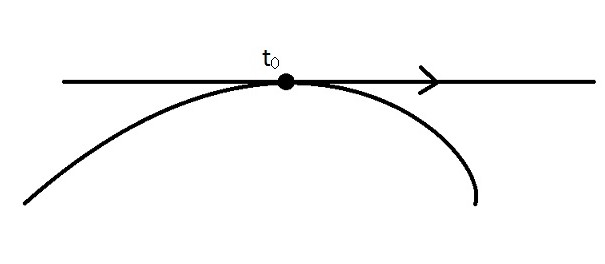
\includegraphics[width = 4.5cm]{tangent}
$\varphi' (t_0) \not = \vec 0$

<- касательная прямая

  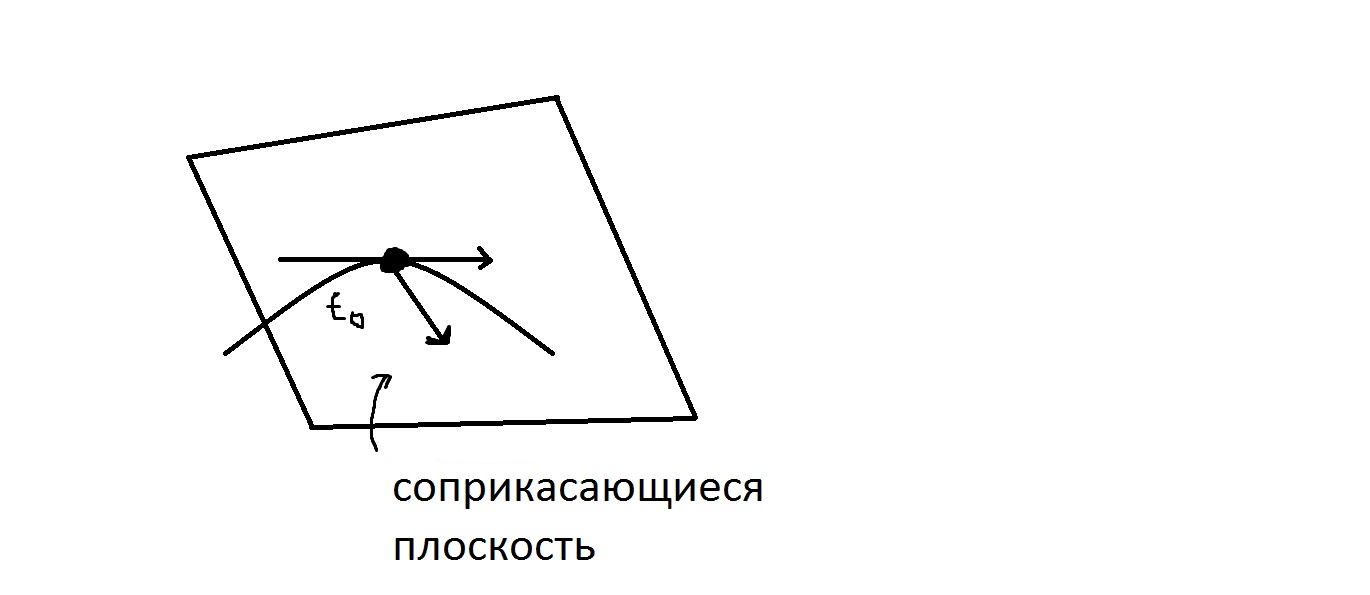
\includegraphics[width = 6cm]{beleg}
$t_0$ называется точкой билигулярности.

$\vec \varphi = \vec p(t)$ называется билигулярной если все ее точки являются
точками билигулярности

  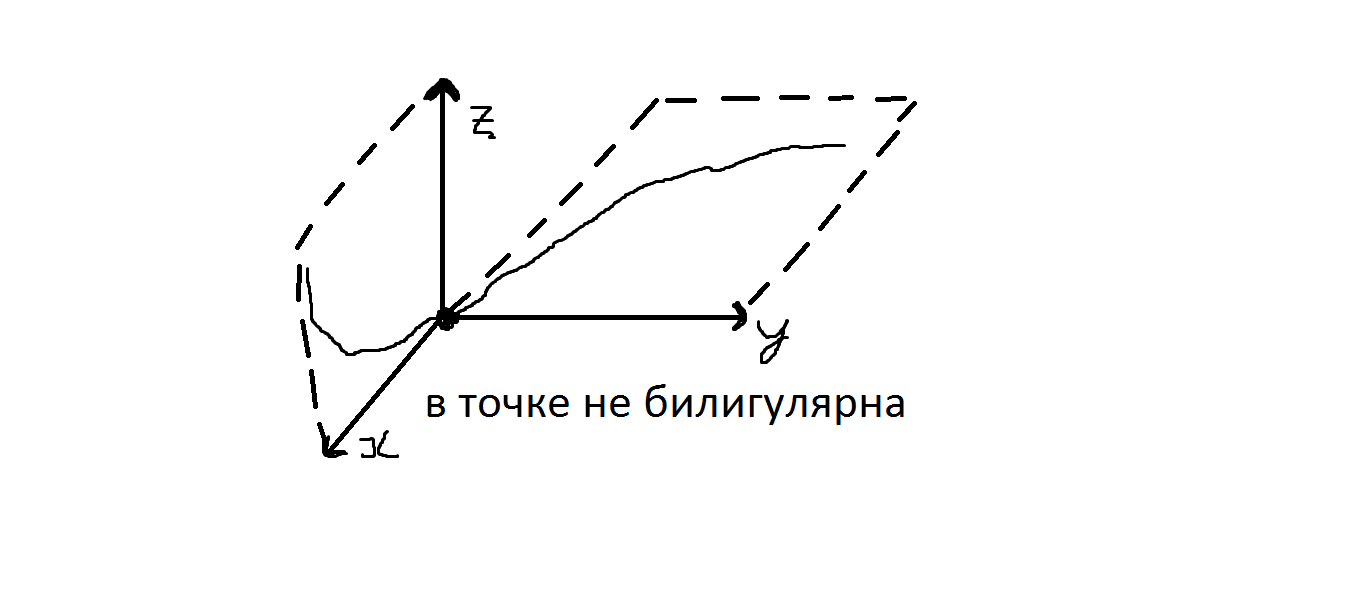
\includegraphics[width = 6cm]{notBeleg}

Пример:
$$
\left\{
\begin{array}{l}
x = a \cos t \\
y = a \sin t
\end{array}
\right.
s = \tg \frac{t}{2} ~~~ \sin t = \frac{2s}{1+s^2} ~~~
\cos t = \frac{1-s^2}{1+s^2} ~~~
\left\{
\begin{array}{l}
x = a \frac{1-s^2}{1+s^2} \\
y = a \frac{2s}{1+s^2}
\end{array}
\right.
$$

Дифоморфизмом называется гладкое отображение при котором обратное отображение
тоже гладкое.

Биективное отображение гладкое в обе стороны.

\begin{define}
  Пусть даны две кривые

  $\varphi_1 : [a,b] \to R^3$

  $\varphi_2 : [a,b] \to R^3$

  Эти кривые называются эквивалентными если существует дифиморфизм
  $\varphi : [a,b] \to [\alpha, \beta]$
\end{define}

Пример:
$$
\varphi_1(t) = (a\cos t, a \sin t)
$$
$$
\varphi_2(t) = (a \frac{1-s^2}{1+s^2}, a \frac{2s}{1+s^2})
$$

Параметризация эквивалентных прямых называется эквивалентными если все кривые
разбиваются на классы эквивалентных кривых эти классы классы эквивалентности
кривых называются не параметрихованными кривыми.